\chapter{Experimental Setups}
\label{ch:exptsetup}

In all experiments in this thesis, a flow circuit was used to contain the blood and provide control over parameters like oxygenation.
This circuit is similar to what is used in cardio-pulmonary bypass surgery, where a patient's blood is pumped and oxygenated by a heart lung machine.
Over the course of this research, the experimental setup was improved, leading to two main versions - the original stopped flow setup, and the continuous flow setup.

\section{Stopped flow experimental setup}
\label{sec:exptsetup-stopflow}

\subsection{Flow circuit and pump}
\begin{figure}[t]
\centering
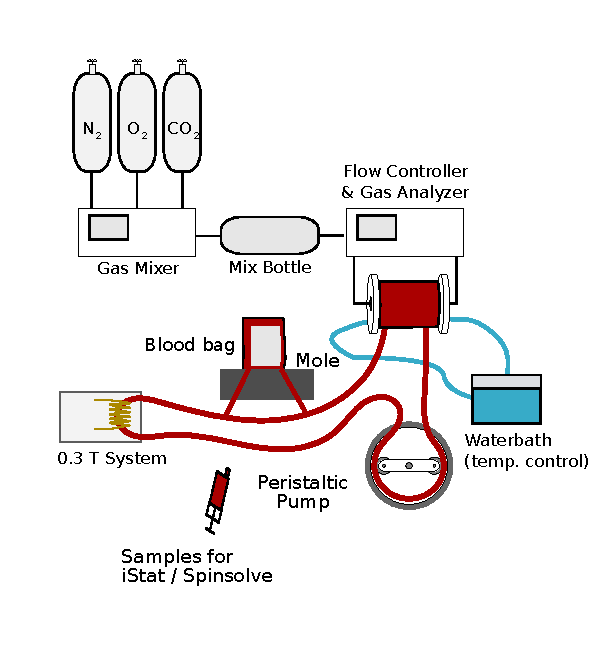
\includegraphics[width=0.75\textwidth]{figures/exptsetup/BloodMixingSetup.pdf}
\caption{Schematic of the Stopped flow setup}
\label{fig:exptsetup-stopflowschematic}
\end{figure}

A schematic of the flow stopped setup is shown in \autoref{fig:exptsetup-stopflowschematic}.
The main components are the roller pump and the oxygenation membrane, with the blood collection bag acting as a reservoir.
These are all joined by 1/4'' medical grade PVC tubing.
The total volume of this circuit was typically \SI{60}{\milli\litre}, with the blood bag containing 450 ml TODO check logbook.

The roller pump is used to generate flow around the circuit, by rotating the pump head to drive 2 rollers that squeeze the walls of the tube and force the blood along.
The pump is also designed for use in CPB surgery, and is a Stockert SIII, with a flow rate controllable from \SIrange{0.01}{6}{L/m} when used with the 1/4'' tube. TODOcheck?.
These versions of the flow circuit included a bypass section controlled by clamping the tubes so that the blood flow could be directed to around the reservoir, allowing for faster changes in the oxygenation due to a lower effective volume.
One important setting on the pump is the occlusion, which controls how much the tubing is squeezed as the pump head rotates.
Having the occlusion set too loosely causes the pump to become ineffective, as the blood can flow backwards through the pump, while setting it too tightly was found to cause damage to the red blood cells as they travel through the pump.
One problem with the model of pump used in these experiments does not have any sort of readout of the occlusion setting, so this had to be set at the correct value by following a testing procedure each time the occlusion was changed.

\subsection{Oxygenator and Gas Mixer}
A hollow-fibre membrane oxygenator was used to control the oxygenation of the blood in the circuit.
This was a Medtronic Affinity Pixie oxygenator, designed for use in paediatric CPB procedures.
It allows for gas exchange and temperature control of the blood flowing through, with the oxygenation controlled by the mix of gases going into the oxygenator.
This paediatric model was chosen to minimize the required priming volume, and it still provided more than enough capacity to oxygenate the blood at the flow rates used.
The temperature of the blood was regulated by flowing water from a temperature controlled waterbath through the oxygenator, which has a separate path built into it for this purpose.
The water bath temperature was set to \SI{35}{\degreeCelsius}, although this corresponded with a blood temperature at the outlet of \SI{33}{\degreeCelsius} at maximum flow rates (with lower temperatures at lower flow rates.)

The gas mix was set using a Dansensor MapMix 3 gas mixer, which allowed control of the different proportions of \Ntwo, \Otwo, and \COtwo flowing through the oxygenator.
The Oxygen fraction was typically varied from 0\% up to 21\%, the value of atmospheric air.
Nitrogen was used as a non-Oxygen containing gas, and between 2.5-5\% \COtwo was also added to ensure the pH of the blood sample remained stable over the course of the experiment (as these are linked by the bicarbonate buffer system in blood).
Gases for all experiments were used as supplied from BOC and were instrument grade or higher.
The output of the gas mixer flowed into a pressurised buffer tank before flowing into a Dansensor MapCheck Provectus gas analyser, which allowed us to check the fraction of the three gases which flowed into the oxygenation membrane.
This gas analyser also provided some flow regulation, although this was supplemented with an adjustable flow valve.
Typically, the gas flow rate was set to only \SIrange[per-mode=symbol]{1}{2}{\liter\per\minute} to avoid creating bubbles in the oxygenator.

\subsection{Blood collection}
Samples of whole blood were collected by venipuncture from healthy volunteers (taking place at Otago medical school).
This procedure was approved by the Central Health and Disability Ethics Committee (15/, and all volunteers provided written, informed consent.
Approximately \SI{450}{ml} of blood was collected into a blood bag containing \SI{66.5}{\milli\litre} CPD anticoagulant/preservative solution (Haemonetics Leukotrap WB system).
CPD solution is rated for storage of red blood cells for up to at least 3 weeks of storage\cite{Hessupdatesolutionsred2006}.
Blood samples were held at room temperature following collection, before undergoing leukoreduction filtering to remove white blood cells, s it has been shown that the presence of white blood cells can adversely affect the condition of red blood cells in storage\cite{Hessupdatesolutionsred2006}.
Samples were then moved to a refrigerator and stored at \SI{4}{\degreeCelsius} until required for experiments (up to 30 TODO check! days for stopped flow experiments, up to 10 days for continuous flow experiments)

\subsection{NMR setup}
For these experiments, 3 different permanent magnet systems were used to obtain data at 3 different field strengths.
TODO pics of magnets!!

The first system was a 12 MHz (\SI{0.3}{T}) Halbach magnet array, with \SI{9}{cm} diameter bore and approximately \SI{20}{\centi\metre} long.
This magnet was repurposed from a previous experiment in the lab, and specifications are not available for it.
When combined with the home built coil and holder system described in \autoref{sec:exptsetup-coil}, the FID linewidth produced by the magnet was \SI{12}{\kilo\hertz}, which is relatively broad.

Because it uses permanent magnets, it requires a stable temperature in order to have a stable field.
This was set up using a temperature controlled water bath, which pumped wat at a constant \SI{30}{\celsius} through tubes wrapped around the magnet.
On top of this, the magnet was wrapped in a layer of foam, and a layer of mylar sheeting to insulate it from the room.
To decrease the effect of electrical noise on the measurements, the magnet assembly was also surrounded by a thin coppper mesh blanket.

The second magnet system used was the NMR MOLE, previously developed by Manz et al\cite{ManzmobileonesidedNMR2006}.
The NMR MOLE operates at a field of \SI{0.1}{T} and is a single sided device, which produces a `sweet spot' in the region above the magnet.
The sweet spot is where the combination of magnetic field and RF produced by the coil on the surface are able to create resonance, which defines where signal comes from.
In this case, the sweet spot was a pair of regions marking out a \SI{3}{cm} circle over the RF coil (TODO see figure? honours project).
While earlier experiments attempted to position the tube containing blood over the sweet spot, in later experiments, it was decided that it was simpler and more reliable to place the blood bag on the top of the MOLE.
As with the Halbach array, the MOLE is also sensitive to temperature, so an electronic temperature controller and wire heater were used to keep it stable at \SI{29}{\celsius}.

The design of the magnet array in the MOLE creates strong magnetic field gradients across the sweet spot.
This creates a wide range of resonance frequencies, and means that it was not possible to measure an FID from the system.
It was also found that this limited the possible range of CPMG echo times, as echo times longer than \SI{1}{ms} were caused excessive signal attenuation.
This limited experiments with this system to short echo times.

The third magnet system used was a Magritek Spinsolve, which is another permanent magnet based NMR system operating at \SI{1}{T}.
The Spinsolve is designed for chemical spectroscopy, so has a very homogeneous field, and can produce a linewidth of less than \SI{0.1}{Hz}.
It also uses standard 5 mm NMR sample tubes, so it could not be used inline in the flow circuit like the other two systems.
Because of this, experiments on the Spinsolve required withdrawing a small amount of blood and transferring it into an NMR tube.
This meant that that there were typically delays between removing the blood from the circuit and taking measurements on it, which may cause changes in the state of the blood.

Both the Halbach and MOLE systems were controlled on computers running Magritek Prospa, and used Magritek Kea 2 spectrometers to run the NMR experiments.
The Spinsolve was also controlled from a computer with a newer version of Prospa.
CPMG experiments were run using the default CPMG macros included in Prospa, with batch scripts set up to automate taking measurements at multiple echo times.

\section{Continuous flow setup}
\label{sec:exptsetup-contflow}

To be able to get better data on how \Ttwo is affected by \SOtwo at different fields, we decided to move to a continuous flow method, where the \SOtwo was slowly ramped from low to high oxygenation, while the \Ttwo was constantly measured.
This required a number of changes to the stopped flow setup, including the use of the baby-MRI magnet, and the development of a system for continuous \SOtwo tracking.


\begin{itemize}
\item Flow Circuit changes
\item different magnet
\item sO2 measurement - optical sensor, calibration
\end{itemize}

\subsection{Flow Circuit Changes}
When first moving on to the measurements using continuous flow, the same flow circuit setup used in the stopped flow experiments was used.
It was found that the design of the circuit, with the pump connected directly in line after the NMR system caused unacceptable variations in the flow rate through the probe, creating spikes in the measurements of \Ttwo (see TODO(continuous flow results?).
This is due to the two roller design of the pump, which means that at a specific point in its rotation, the flow rate drops.
To remedy this issue, the circuit was rearranged to include an additional empty blood bag between the magnet and the pump.
A steady flow rate was generated by allowing blood to flow under gravity, with the flow regulated with a screw clamp.
The screw clamp was set at the beginning of the experiment to give a flow rate of \SIrange{1}{2}{cm/s}, which was measured by PGSE experiments.
This gave a stable flow rate and constant \Ttwo measurements.

Additionally, the bypass section was removed from the circuit.
It was found that portions of the blood would stagnate in this section and in the Y-joints and flow into the main circuit at random.
As the oxygen saturation in the main circuit was changing, the blood in this section would lag behind and cause pockets of blood with different oxygenation to flow through the main circuit, which disrupted the gentle ramps in \SOtwo that were generated by the oxygenator and upper reservoir.

The remaining parts of the flow circuit, including the oxygenator, gas mixers, and sampling methods remained the same from the stopped flow experiments.
Additional thermal insulation was added to the tubing and blood bags to improve temperature stability.
A diagram of the continuous flow version of the circuit is included in \autoref{fig:exptsetup-contflow-schematic}.

\begin{figure}[t]
\centering
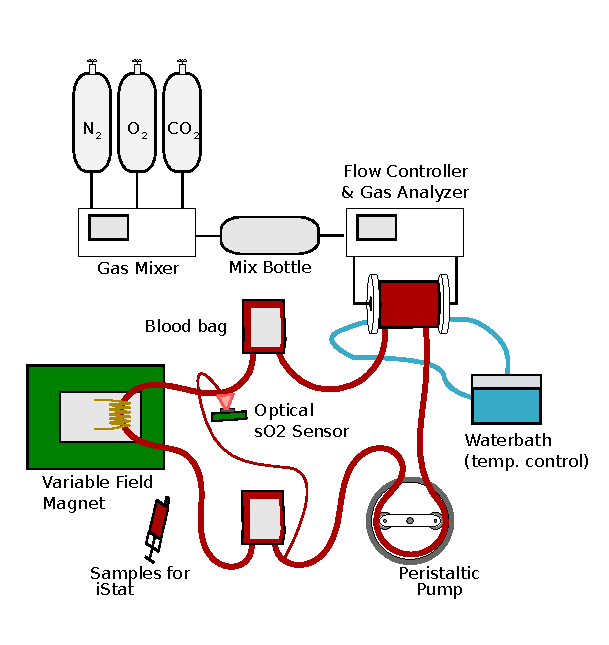
\includegraphics[width=0.75\textwidth]{figures/exptsetup/contflowschematic.pdf}
\caption{Schematic of the continuous flow circuit}
\label{fig:exptsetup-contflow-schematic}
\end{figure}

\subsection{Baby-MRI magnet}
After the difficulties in working with the permanent magnet system, the research moved onto the baby-MRI magnet.
This is a cryogen-free magnet system (Cryogenic Limited, London UK), where the field can be changed from \SI{0}{1.5}{T} by adjusting the current in the superconducting coils.
The bore has a diameter of \SI{8}{cm}, and is \SI{60}{cm} long.
The magnetic field it generates is much more homogneous than the permanent magnet systems, and it was possible to neasure an FID with a \SI{100}{Hz} linewidth.
It also has a 3-axis gradient coil set, which allows it to be used for imaging and PGSE experiments.

The experiments were controlled by a Kea 2 NMR spectrometer (Magritek, Wellington NZ) with a gradient controller.
An external RF amplifier (American Microwave Technologies) is used, along with Bruker BAFPA-40 gradient power amplifiers (Bruker, Billerica, MA USA).
These were used with the custom built probe, tuning and matching circuit and RF coils described in \autoref{sec:exptsetup-coil}.
To help stabilise the sample temperature, the gradient set was warmed by flowing water through the cooling water tubes from a water bath set to \SI{28}{\celsius}.

It was also discovered that the magnet power supply unit (used to change the magnet current and field strength) creates interference which disrupted NMR experiments.
This occured when echo times were approximately \SIrange{8-12}{ms}, and caused CPMG echo trains that were not exponential decays.
While the exact cause of this effect is unknown, it was removed by ensuring the magnet power supply was switched off during measurements.

\subsection{Coil Assemblies and Electronics}
\label{sec:exptsetup-coil}
A new coil holder, coil assembly and tuning and matching circuit was designed to fit into the baby-MRI system and also used in the Halbach magnet array experiments in  \autoref{ch:stoppedflow}.
It was designed with exchangeable coils and tuning and matching capacitors so that the probe could be tuned and matched at multiple fields / frequencies.
It consists of a probe (outer piece), which holds the coil assembly and the tuning and matching circuit inside the bore of the magnet (which had the same diameter in the two magnets).

The coils are \SI{2}{cm} long, and have a diameter of \SI{1}{cm}, so that the 1/4'' tube can be passed through the coil,
Different numbers of turns were used for the three different coils, to be able to use the coils at different frequencies (More turns causes more inductance, and a lower resonant frequency.)
In the initial design of the coil assembly, the coil was constructed from \SI{0.67}{mm} Copper wire wrapped around a rolled up acetate cylinder.
A second version of the coil assemblies used 3D printed forms made from ABS plastic (to decrease unwanted signal), with the same wire and number of turns.

TODO:picture of the coils and boards
TODO:picture of the T\&M circuit

The tuning and matching circuit was also designed and manufactured for this probe.
It allows for the capacitors to be exchanged, using small PCBs with different capacitors attached.
The circuit also contains variable capacitors which are used for fine tuning the match frequency.
While the higher frequencies only require small changes in capacitance to be tuned and matched using only the variable capacitors (\SIrange[range-phrase = --]{40}{60}{MHz} can be tuned with \SI{20}{pF} or less from the variable capacitors), tuning and matching to lower frequencies required much higher capacitance and inductance.
Switching the different capacitors allowed the probe to be tuned and matched at frequencies ranging from \SIrange{2}{60}{\mega\hertz}.

As the probe is located inside the magnet, the capacitors are all of a non-magnetic type (AVX Hi-Q (AVX, Greenville SC US)  or MCM series (Cornell Dubilier CDE, New Bedford MA US) and are also rated for high voltage (\SI{>500}{V}.)

\textit{S\textsubscript{11}} simulations were run in Qucs Spice to find the approximate values of C\textsubscript{T} and C\textsubscript{M} at a range of frequencies with the different coils.
These were then used to find the configurations in \autoref{tbl:exptsetup-capconf} for the tuning and matching circuit that were used in experiments.
The configurations were tested by measuring \textit{S\textsubscript{11}} on a spectrum analyser, before attaching to the Kea for wobbling.

\begin{table}[ht]
\centering
\begin{tabular}{|c|c|c|}
\hline
Frequency (\si{MHz}) & Coil & Capacitor board\\
\hline
40 & A (8 turn) & 4.7/1 \\
20 & A (8 turn) & Switched 63 \\
14 & C (10 turn) & Switched 33+18 \\
10 & C (10 turn) & 100/12 \\
5.2 & E (14 turn) & 220/24 \\
\hline
\end{tabular}
\caption{Tuning and matching settings used in the continuous flow experiments}
\label{tbl:exptsetup-capconf}
\end{table}

\subsection{Optical \SOtwo measurement}
Making measurements with continuously flowing blood required continuous monitoring of the \SOtwo of the blood going into the magnet system.
This meant that the iStat would not be suitable for these experiments, due to the cost of the cartridges and the length of time it took to measure each sample (approximately two minutes.)
While there were a number of possible techniques for this such as polarographic or fibre-optic p\Otwo sensors, it was decided to use an optical/NIR setup.

This optical system was designed around the MAX30102 sensor (Maxim Integrated, San Jose CA US), which is an integrated pulse oximetry/heart rate module.
It contains all the components for two wavelength pulse oximetry including a \SI{660}{nm} red LED, a \SI{880}{nm} IR LED, LED driver circuits, a photodiode and 18-bit ADC, and a digital ambient light cancellation filter.
The sensor is included on an evaluation board (MAXREFDES117) (Maxim Integrated, San Jose CA US), which includes a voltage regulator and level shifter to allow it to be connected and supplied from 5V electronics.

The sensor measures the red and IR light reflected by the blood by alternately pulsing the red and IR LEDs and measuring the photodiode output.
In this experiment, the LED pulse time was \SI{411}{\micro\second} (the longest possible value to get the most sensitivity), and the sample rate set to \SI{100}{Hz} with a 4x averaging filter to give 25 samples per second.
Other parameters were set to the suggested values in the evaluation demo.
The MAX30102 sensor communicated over I\textsuperscript{2}C to an Arduino board, that reads the incoming data and sends to to the computer to be logged over USB.
This data is collected by a Python application, which provides a live plot of the data from the sensor and averages it further (100x) to reduce the amount of data stored.
The application saves values of the red intensity, IR intensity every 4 seconds.

As discussed in (TODO background-pulseoximetry), the ratio of red and IR intensities are typically converted to \SOtwo using an empirical calibration curve.
To create this curve, samples were collected while the oxygenation was being decreased, the \SOtwos measured using the iStat.
The ratio for each sample was also measured, and used to fit a quadratic curve to find \SOtwo as a function of \textit{R}.
The procedure for this process improved over the course of the experiments, to try and ensure that what was sampled from the circuit and tested on the iStat was on the sensor at the time it the ratio was measured.

To get a good distribution of data points across \textit{R}, samples were taken every 0.1 units, approximately 2.5 corresponds to oxygenated blood,and 0.3 is completely deoxygenated.
Before sampling, approximately \SI{2}{ml} was syringed from the sample tube (thin tube in \autoref{exptsetup-contflow-schematic}) and flushed to the other bag by syringe to remove the volume of the tube.
A \SI{0.5}{ml} sample was taken and measured as soon as possible on the iStat.
When this was not immediately possible, samples were capped with parafilm to try and avoid any changes in \SOtwo due to absorbing Oxygen from the air.
